\documentclass{article}
\usepackage{graphicx}

\usepackage{titling}
\newcommand{\subtitle}[1]{%
  \posttitle{%
    \par\end{center}
    \begin{center}\large#1\end{center}
    \vskip0.5em}%
}

\begin{document}

\title{Software Entwicklung Projekt - Sonjas Coursera - Use Case Diagramm}
\subtitle{Allgemeine Informatik - IN7 - Prof. Dr. Jobst}
\author{Sonja Riethig}

\maketitle

\begin{abstract}
Das Projekt "Sonjas Coursera" implementiert einen einfachen Online-Kurs - Anbieter. Im Folgenden werden die Anforderungen an das Projekt mithilfe von Diagrammen mit Anmerkungen dargestellt.
\end{abstract}

\section{Use Case Diagramm}

\begin{figure}
    \centering
    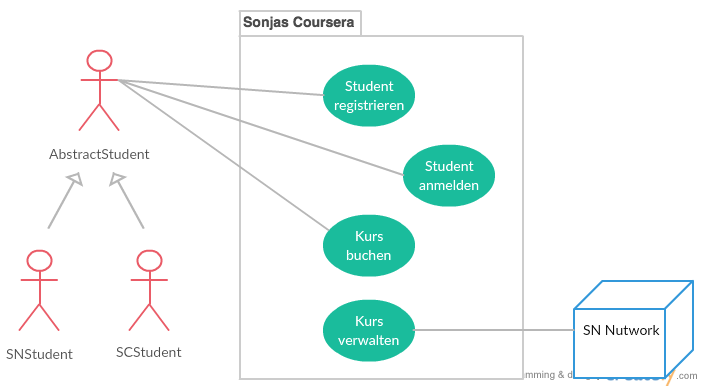
\includegraphics[width=15cm]{../images/SonjasCoursera-UseCaseDiagram.png}
    \caption{Klassendiagramm}
    \label{Klassendiagramm}
\end{figure}

\section{Details der Use Cases}

\subsection{Student registrieren}

\subsection{Student anmelden}

\subsection{Kurs buchen}

\subsection{Kurs verwalten}

\end{document}